\documentclass{scribe-cgenomics}
\usepackage{float}
\usepackage{subfig}
\usetikzlibrary{matrix, positioning}

\begin{document}

\جلسه
{دکتر کسری علیشاهی، ترم دوم سال تحصیلی ۱۴۰۰}
{تمرین شبیه‌سازی}
{محسن قدرتی}

\newpage
\section{}
ابتدا یک بردار تصادفی از سایز
$k$
از توزیع نرمال استاندارد می‌سازیم و آن را
$X$
می‌نامیم. اکنون بردارهای تصادفی رکورد تا لحظه
$k$ام
($R_k$)
 و تعداد رکوردشکنی‌ها تا لحظه
$n$ام
($N_k$)
دارای ضوابط زیر هستند:

\begin{center}
$
\begin{cases}
R_k = \max (X_1, \dots, X_k) \\
N_k = N_{k-1} + \delta_{X_k > R_{k-1}}
\end{cases}
$
\end{center}

نتایج حاصل از ۱۰۰۰ مرتبه تکرار شبیه‌سازی مساله به صورت زیر خواهد بود:

\begin{figure}[h]\label{1}
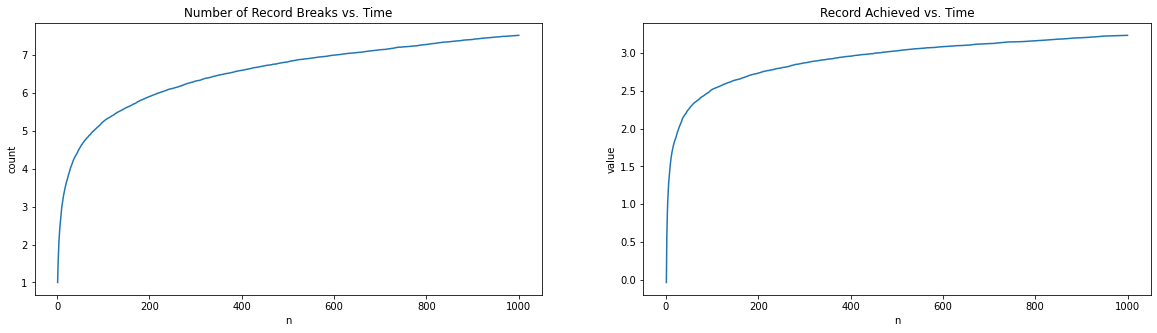
\includegraphics[width=6.5in]{1.png}
\centering
\end{figure}

از روی نمودار، با کمی آزمون و خطا می‌توان نتیجه گرفت که احتمالا:

\begin{center}
$
\begin{cases}
R_k \propto \log k \\
N_k \propto \log k
\end{cases}
$
\end{center}

یا به عبارت دیگر، حدس می‌زنیم متغیر تصادفی
$R_k$
توزیع نمایی، و متغیر تصادفی
$N_k$
نیز توزیع پواسون دارد.


\newpage
\section{}
یک نمونه‌گیری با جایگذاری از سایز
$n$
از توپ‌های ظرف انجام می‌دهیم. سپس در هر گام
$k$،
بردار
$counts_k$
شامل تعداد مشاهدات هر گوی در نمونه‌گیری را تشکیل می‌دهیم. توجه می‌کنیم که در هر گام تنها یک درایه از بردار
$counts_k$
بروزرسانی می‌شود. سپس تعداد درایه‌هایی که برابر با یک هستند را می‌شماریم و متغیر تصادفی
$N_k$
را مقدار‌دهی می‌کنیم.  نمودار زیر نتیجه حاصل از اجرای این فرآیند را به ازای ۱۰۰۰ مرتبه نمونه‌گیری نشان می‌دهد:

\begin{figure}[h]\label{2}
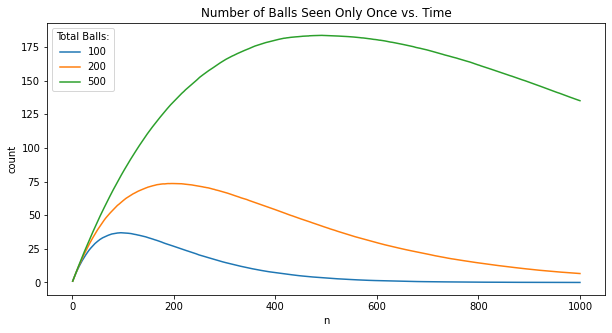
\includegraphics[width=5in]{2.png}
\centering
\end{figure}


\newpage
\section{}
اگر متغیر تصادفی محل شکسته شدن چوب را با
$X$
نشان دهیم، و نسبت طول قطعه بزرگ‌تر به کوچک‌تر را با
$R$،
خواهیم داشت:

\begin{center}
$
R = \dfrac{\max{(X, 1-X)}}{\min{(X, 1-X)}}\..
$
\end{center}

با توجه به این که برای تقریب
$R$
با میانگین نمونه‌گیری، ممکن است نویزهای بسیار شدید ایجاد شوند، در شکل زیر، چند مرتبه نمونه‌گیری انجام داده‌ایم و در نمودار سمت راست، می‌توان میانگین این میانگین‌ها را به همراه بازه عدم قطعیتشان مشاهده کرد.

\begin{figure}[h]\label{3}
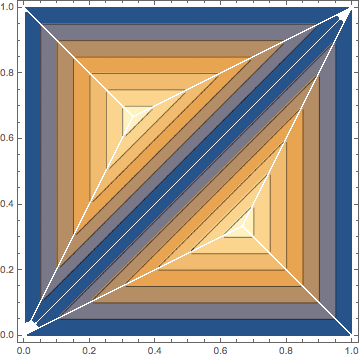
\includegraphics[width=6.5in]{3.png}
\centering
\end{figure}

بر اساس نمودارهای بالا مشاهده می‌شود که نسبت طول قطعه بزرگ‌تر به کوچک‌تر عددی در حدود
$25 \pm 10$
است.


\newpage
\section{}
هر بیضی نمونه‌گیری شده مطابق با فرض مساله، به صورت زیر به شکل یکتا در صفحه قرار می‌گیرد:

\begin{center}
$
\begin{cases}
C := (C_X, C_Y) \sim U[0, 2]^2 & \text{مختصات مرکز بیضی} \\
\theta \sim U[0, \pi] & \text{زاویه بین قطر به طول $\alpha$ با محور افقی} 
\end{cases}
$
\end{center}

اگر معادله نقاط بیضی به صورت زیر باشد:

\begin{center}
$
f:\ ax^2 + bxy + cy^2 -d = 0
$
\end{center}

آنگاه دورترین خطوط افقی و عمودی که با این بیضی تلاقی می‌کنند، نقاطی است که در آنها مشتقات جزیی
$f$
نسبت به
$x$
و
$y$
برابر با صفر است. یعنی:

\begin{center}
$
\dfrac{\partial f}{\partial x} = 2ax + by = 0 
$

$
\implies x^* = \dfrac{-b}{2a}y^*
$

$
\implies a(\dfrac{b^2}{4a^2}){y^*}^2 + b(\dfrac{-b}{2a}){y^*}^2 + c{y^*}^2 - d = 0
$

$
\implies {y^*}^2 \big( \dfrac{b^2}{4a} - \dfrac{b^2}{2a} + c \big) = d
$

$
\implies {y^*}^2 (c - \dfrac{b^2}{4a}) = d
$

$
\implies {y^*}^2 = \dfrac{4ad}{4ac - b^2}
$
\end{center}

پس به طریقی مشابه، بعد از یافتن فرمول مشابهی برای مرزی‌ترین نقاط افقی بیضی مذکور، کلیه نقاط بیضی درون محدوده

\begin{center}
$
C_X \pm \sqrt{\dfrac{4cd}{4ac-b^2}}, \quad
C_Y \pm \sqrt{\dfrac{4ad}{4ac-b^2}}
$
\end{center}

قرار می‌گیرند.

اکنون توجه می‌کنیم که معادله بیضی هنگامی که زاویه قطر به طول
$\alpha$
آن با محور افقی برابر با صفر باشد، به صورت زیر است:

\begin{center}
$
x^2 + \alpha^2 y^2 = \dfrac{\alpha^2}{4}
$
\end{center}

اما معادله نقاط بیضی پس از دوران به اندازه
$\theta$
عبارت است از:
$R_{\theta} 
\begin{bmatrix}
x \\ y
\end{bmatrix}
 = \begin{bmatrix}
 X \\ Y
 \end{bmatrix}
 $
 که در آن
 $R_{\theta}$
 ماتریس دو بعدی دوران مرسوم است. در نتیجه نقاط صادق در بیضی دوران یافته در معادلات زیر صدق می‌کنند:
 
\begin{center}
$
\begin{cases}
x = \cos \theta X + \sin \theta Y \\
y = -\sin \theta X + \cos \theta Y
\end{cases}
$
\end{center}

که با جایگذاری در معادله اولیه، معادله بیضی دوران یافته به اندازه
$\theta$
به شکل زیر به دست می‌آید:

\begin{center}
$
(\cos \theta X + \sin \theta Y)^2 + \alpha^2 (-\sin \theta X + \cos \theta Y)^2 = \dfrac{\alpha^2}{4}
$

$
\implies X^2(\cos^2 \theta + \alpha^2 \sin^2 \theta) + 
XY (2\sin \theta \cos \theta - 2\alpha^2 \sin \theta \cos \theta) + 
Y^2 (\sin^2 \theta + \alpha^2 \cos^2 \theta) - \dfrac{\alpha^2}{4} = 0
$
\end{center}

در نتیجه

\begin{center}
$
\implies 4ac - b^2 = 4 (\cos^2 \theta \sin^2 \theta + \alpha^2 \cos^4 \theta + \alpha^2 \sin^4 \theta + \alpha^4 \sin^2 \theta \cos^2 \theta) - 4\sin^2 \theta \cos^2 \theta (1 + \alpha^4 -2\alpha^2)
$

$
= 4 \alpha^2 (\sin^4 \theta + \cos^4 \theta + 2\sin^2 \theta \cos^2 \theta) = 4\alpha^2
$
\end{center}

پس

\begin{center}
$
x_{\max} = \dfrac{\sqrt{\sin^2 \theta + \alpha^2 \cos^2 \theta}}{2}, \qquad
y_{\max} = \dfrac{\sqrt{\cos^2 \theta + \alpha^2 \sin^2 \theta}}{2}
$
\end{center}

پس شبیه‌سازی به این شکل خواهد بود که متغیر‌های تصادفی با توزیع یکنواخت
$\theta$
و
$C$
را تولید می‌کنیم و سپس بررسی می‌کنیم که آیا
$C_X \pm x_{\max}$
و
$C_Y \pm y_{\max}$
بین صفر و دو قرار دارند یا خیر. اگر همه شروط صادق بودند، یعنی بیضی نمونه‌گیری شده کاملا داخل یک مربع دو  در دو قرار دارد و در صورت نقض حتی یکی از شروط بیان شده نتیجه می‌شود بیضی نمونه‌گیری شده با یکی از محورها تلاقی داشته است.

شکل زیر نتیجه حاصل از نمونه‌گیری‌های از سایز ۱۰۰۰۰ را به ازای چند انتخاب مختلف از طول ضلع مربع‌های مشبکه نشان می‌دهد:

\begin{figure}[h]\label{4}
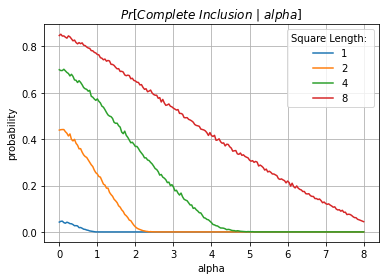
\includegraphics[width=3.5in]{4.png}
\centering
\end{figure}


\newpage
\section{}
برای شبیه‌سازی توزیع
$Pr(X_n | X_{n-1})$
به اندازه
$X_{n-1}$
متغیر تصادفی یکنواخت استاندارد تولید می‌کنیم و سپس با مقایسه هر کدام با احتمال دوفرزندی شدن
$p$،
اگر مقدار متغیر تولید شده در بازه
$[0,\ p]$
بود، یک و در غیر اینصورت صفر جایگذاری می‌کنیم. سپس مجموع متغیرهای تصادفی را ضرب در دو می‌کنیم و به این شکل
$X_n$
نمونه‌گیری می‌شود.


اکنون در شکل زیر که حاصل از ۲۰۰۰۰ بار شبیه‌سازی فرآیند شاخه‌ای با روش نمونه‌گیری فوق است، در می‌یابیم که به ازای
$1-p = 0.5$
نسبت به
$1-p = 0.501$
میانگین کمی بزرگ‌تر است و انحراف معیار نیز کمی بیشتر است. به عبارت دیگر، متوسط زمان انقراض در تناسب با افزایش احتمال عقیم بودن یک راس کاهش می‌یابد. 

در واقع نمودار‌های سمت راست کمی به صفر متمایل‌تر هستند و در عوض نمودار‌های سمت چپ کمی از صفر پراکنده‌تر هستند.

نکته قابل توجه آن است که برای اینکه نمودار‌های ردیف بالا، قابل رسم باشند، تصمیم گرفتیم مقادیر بزرگتر از یک آستانه را در یک بازه انتهای شکل جمع کنیم. که این موضوع باعث شده است تفاوت دو حالت به چشم نیاید و حتی میانگین زمان انقراض در
$p = 0.5$
کمتر از حالت دیگر باشد که خلاف شهود و نتیجه ردیف پایینی  (مقیاس لگاریتمی زمان انقراض) است.

\begin{figure}[h]\label{5}
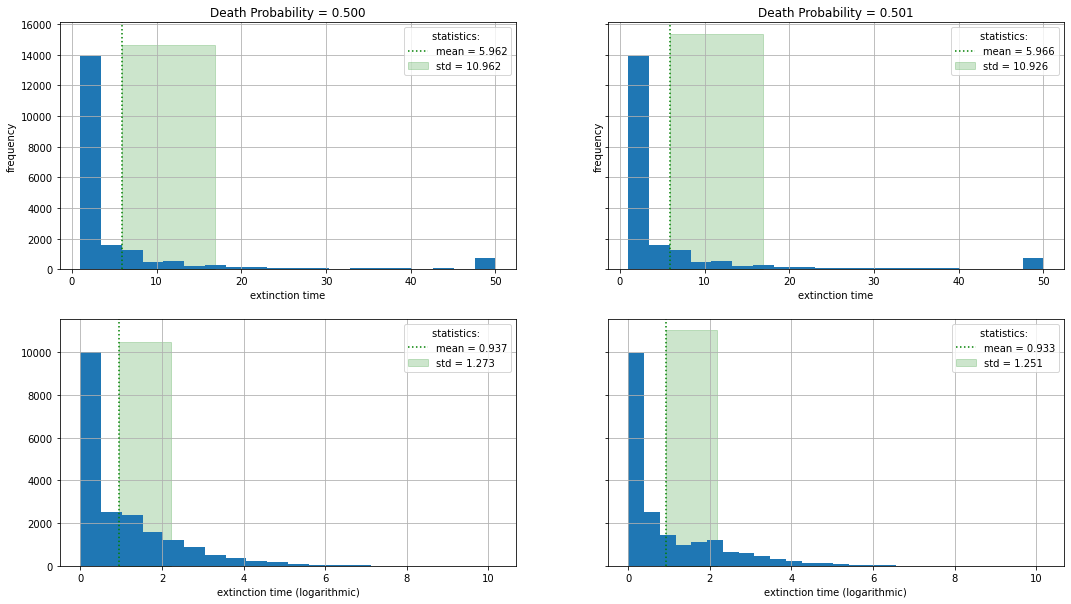
\includegraphics[width=6.5in]{5.png}
\centering
\end{figure}


\newpage
\section{}
ماتریس انتقال فرآیند مارکف مدل به شکل زیر است:

\begin{center}
$
P = \begin{bmatrix}
0 & 1-p & \dots & p\\
p & 0 & 1-p & \vdots \\
\vdots & \ddots & 0 & \ddots \\
1-p & \dots & p & 0
\end{bmatrix}
$
\end{center}

توجه می‌کنیم که به ازای
$n$های
زوج، زنجیر مارکف مورد نظر متناوب است (بین حضور در خانه‌های زوج و فرد). پس تنها به ازای مقادیر فرد، فرآیند مورد نظر را بررسی می‌کنیم.

هیستوگرام حاصل به شکل زیر است:

\begin{figure}[h]\label{6a}
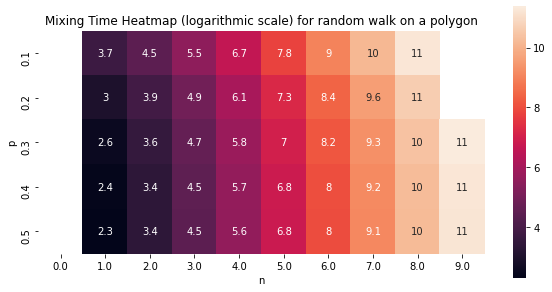
\includegraphics[width=4in]{6a.png}
\centering
\end{figure}

برای افزایش سرعت محاسبات، توجه می‌کنیم که به جای استفاده از ماتریس انتقال، می‌توان به این نکته توجه کرد که بردار حالت در هر لحظه، از ترکیب بردار حالت در لحظه قبل با یک شیفت به چپ و یک شیفت به راست تشکیل می‌شود. در واقع:

\begin{center}
$
\sigma_{n+1} = p \sigma_n ^{\leftarrow} + (1-p) \sigma_n ^{\rightarrow}
$
\end{center}

همانطور که در نمودار‌های زیر مشهود است، به ازای یک 
$n$
ثابت، مربع وارون نرم (بی‌نهایت) بردار حالت با تعداد ایتریشن‌ها رابطه مستقیم دارد (تا وقتی به زمان آمیختگی برسیم، این رابطه حفظ می‌شود و سپس نمودارها افقی خواهند شد). یعنی زمان آمیختگی را می‌توان با متغیرهای پیوسته زیر که رابطه‌ای خطی با آن دارند جایگزین کرد:


\begin{center}
$
T \propto \dfrac{1}{|| \sigma_T - \pi||_{\infty}^2}
\quad \text{برای $n$ ثابت:}
$
\end{center}


در واقع انتظار داریم منحنی‌ها تا جایی به صورت خطوط با شیب ثابت حرکت کنند و سپس از جایی به بعد به خطوط افقی تبدیل شوند (چون نرم بی‌نهایت بردارهای حالت از جایی به بعد (در حوالی زمان آمیختگی) ثابت می‌شود و لذا مربع وارون آن نیز ثابت خواهد شد.

\bigbreak

نمودار به ازای
$n=1001$
ثابت و
$p$های
متفاوت:

\begin{figure}[h]
\subfloat[]{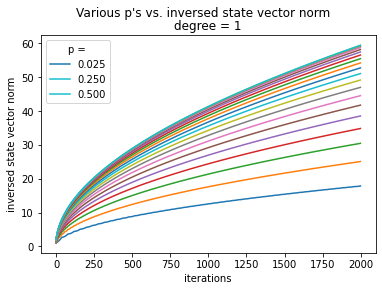
\includegraphics[width = 2in]{6b1.png}} 
\subfloat[]{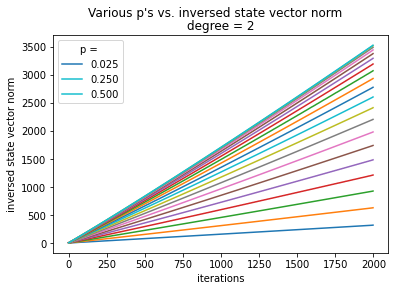
\includegraphics[width = 2in]{6b2.png}} 
\subfloat[]{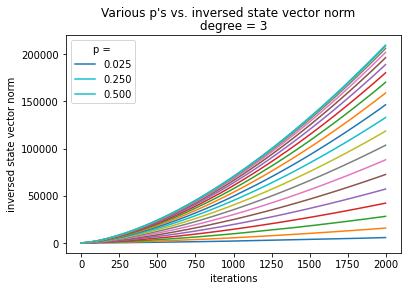
\includegraphics[width = 2in]{6b3.png}}  
\label{6_p_relation}
\centering
\end{figure}


به همین ترتیب نمودارهای زیر نشان می‌دهند به ازای یک
$p$
ثابت، لگاریتم نرم بی‌نهایت بردار باقیمانده با تعداد ایتریشن‌ها رابطه مستقیم دارد. یعنی

\begin{center}
$
T \propto \log|| \sigma_T - \pi||_{\infty}
\quad \text{برای $p$ ثابت:}
$
\end{center}

نمودار به ازای سه مقدار ثابت
$p \in \{0.1, 0.3, 0.5 \}$
و
$n$های
متفاوت:

\begin{figure}[h]\label{6_n_relation}
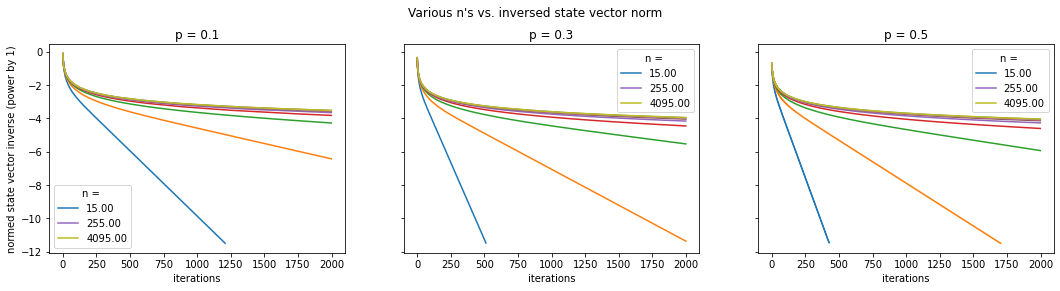
\includegraphics[width=6.5in]{6c.png}
\centering
\end{figure}

اکنون با مقایسه مقادیر مختلف
$n$
و
$p$
و با فرض ثابت بودن دیگری، نمودارهای زیر را خواهیم داشت که رابطه تابعی از نرم بی‌نهایت بردار باقیمانده را به ازای
$T = 100000$
مرحله ادامه آمیختن، با مقادیر مختلف
$n$
و
$p$
نشان می‌دهد. از طرفی در نمودارهای قبل نشان دادیم که این روابط، روابط مشابهی بین زمان آمیختگی و
$n$
و
$p$
را نیز نتیجه می‌دهند.

\begin{figure}[h]
\subfloat[رابطه لگاریتمی]{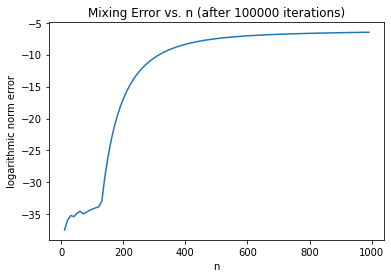
\includegraphics[width = 3in]{6d.png}} 
\subfloat[رابطه تقریبا خطی]{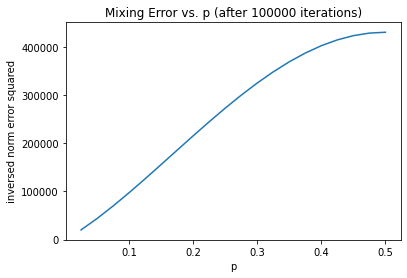
\includegraphics[width = 3in]{6e.png}} 
\label{6_relations}
\centering
\end{figure}


پس به طور تقریبی بر اساس نمودارهای فوق:

\begin{center}
$
T_{mixing} \propto \max(p, 1-p),
\qquad
T_{mixing} \propto \exp(n)
$
\end{center}

\newpage
\section{}


فرض کنیم یک چنبره
$n\times n$
در اختیار داریم. اگر متغیر تصادفی
$\theta(X,Y)$
را برابر با زمان رسیدن از نقطه
$X$
به
$Y$
در نظر بگیریم، هدف مساله یافتن مقدار زیر است:

\begin{center}
$
E_Y[\theta (X, Y) | X]
$
\end{center}

که به دلیل تقارن مساله، معادل مقدار زیر است:

\begin{center}
$
E_Y[\theta (Y)]
$
\end{center}

که در آن
$\theta(Y)$
زمان رسیدن از نقطه
$(0,0)$
به
$Y$
است.

برای یافتن این مقدار، با شروع از خانه
$(0,0)$
تا زمانی قدم زدن تصادفی را ادامه می‌دهیم که همه خانه‌های چنبره دیده شوند و اولین زمان مشاهده هر خانه چنبره را در یک ماتریس
$M$
یادداشت می‌کنیم. اکنون این فرآیند را
$10000$
مرتبه تکرار می‌کنیم و ماتریس میانگین‌های
$\bar{M}$
را تشکیل می‌دهیم. در نهایت میانگین مقادیر ماتریس
$\bar{M}$
را گزارش می‌کنیم.


\begin{figure}[h]\label{7}
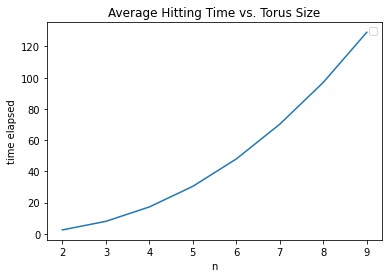
\includegraphics[width=3.5in]{7a.png}
\centering
\end{figure}

در شکل زیر نیز می‌توان گرمانگاری از مقادیر درایه‌های ماتریس
$\bar{M}$
به ازای یک چنبره
$9 \times 9$
مشاهده کرد.

\begin{figure}[h]\label{7hist}
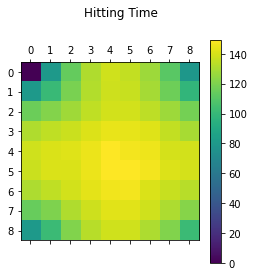
\includegraphics[width=3in]{7b.png}
\centering
\end{figure}

\newpage
\section{}

برای یافتن پاسخ این بخش مشابه بخش قبل عمل می‌کنیم. با این تفاوت که این بار، زمانی که هر ماتریس
$M$
به طور کامل مقداردهی می‌شود را ذخیره می‌کنیم. نمودار زیر به ازای
$n$های
مختلف، مقدار متوسط زمان پوشش را به دست می‌دهد:

\begin{figure}[h]\label{8}
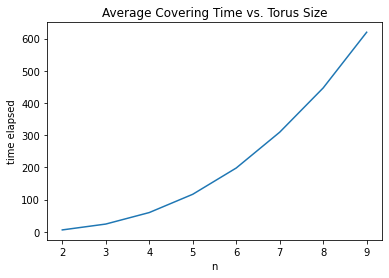
\includegraphics[width=3.5in]{8a.png}
\centering
\end{figure}

در شکل زیر می‌توان منحنی‌های متوسط زمان پوشش و متوسط زمان برخورد را با یکدیگر مقایسه کرد:


\begin{figure}[h]\label{8_comp}
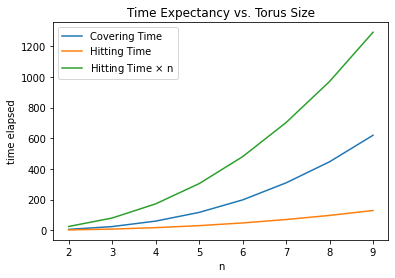
\includegraphics[width=3.5in]{8b.png}
\centering
\end{figure}

\newpage
\section{}
مشابه مساله ۶، به جای استفاده از ماتریس انتقال فرآیند، از رابطه بازگشتی استفاده می‌کنیم. اگر توزیع احتمال فرآیند را در گام
$t$ام 
با
$\sigma_t$
نشان دهیم، داریم:

\begin{center}
$
\sigma_{t+1} = 
\dfrac{1}{4} \sigma_{t}^{\leftarrow} + 
\dfrac{1}{4} \sigma_{t}^{\rightarrow} + 
\dfrac{1}{4} \sigma_{t}^{\uparrow} + 
\dfrac{1}{4} \sigma_{t}^{\downarrow} 
$
\end{center}

هم‌چنین مجددا توجه می‌کنیم که به ازای
$n$های
زوج، زنجیر مارکف مذکور متناوب است، پس تنها حالاتی که
$n$
فرد باشد را بررسی می‌کنیم.

نمودارهای زیر رابطه بین زمان آمیختگی را با سایز چنبره نمایش می‌دهند. تنها تفاوت دو نمودار آن است که در نمودار صمت راست، مقیاس محور عمودی، رادیکالی است. 

\begin{figure}[h]\label{9}
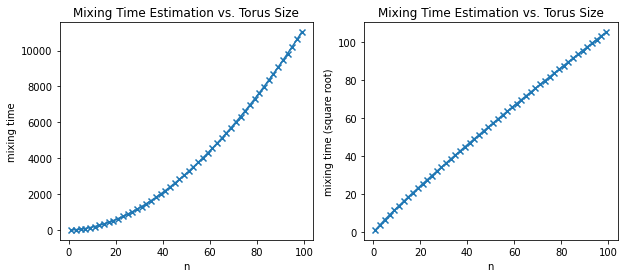
\includegraphics[width=4.5in]{9.png}
\centering
\end{figure}

همان‌طور که از شکل به نظر می‌رسد، حدس می‌زنیم:

\begin{center}
$T_{mixing} \propto n ^ 2$
\end{center}


\newpage
\section{}

مدل نشت جهت‌دار یالی توسط ماتریس زیر قابل بیان است. در این ماتریس، خانه‌های خاکستری همان راس‌های عمق‌های مختلف هستند و عمق برابر است با شماره قطر فرعی شامل راس‌های خاکستری. 

\begin{center}
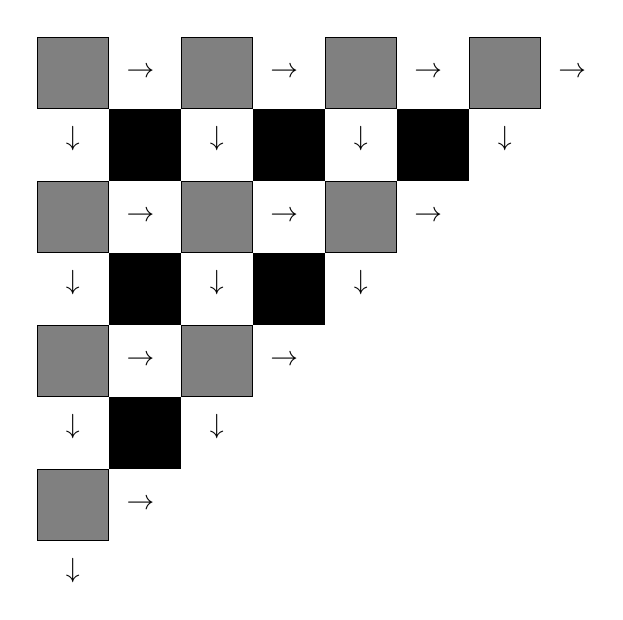
\begin{tikzpicture}
\matrix (A) [matrix of nodes,
    nodes={draw, fill, minimum size=9mm}]
    {|[fill=gray]|~&&|[fill=gray]|~&&|[fill=gray]|~&&|[fill=gray]|~&\\
    &|[fill=black]|~&&|[fill=black]|~&&|[fill=black]|~&&\\
    |[fill=gray]|~&&|[fill=gray]|~&&|[fill=gray]|~&&&\\
    &|[fill=black]|~&&|[fill=black]|~&&&&\\
    |[fill=gray]|~&&|[fill=gray]|~&&&&&\\
    &|[fill=black]|~&&&&&&\\
    |[fill=gray]|~&&&&&&&\\
    &&&&&&&&\\
    &&&&&&&&\\};
    \foreach \i in {1,3,5,7}{ 
        \node[right=1mm of A-1-\i]{$\rightarrow$};
        \node[below=1mm of A-\i-1]{$\downarrow$};}
    \foreach \i in {1,3,5}{ 
        \node[right=1mm of A-3-\i]{$\rightarrow$};
        \node[below=1mm of A-\i-3]{$\downarrow$};}
    \foreach \i in {1,3}{ 
        \node[right=1mm of A-5-\i]{$\rightarrow$};
        \node[below=1mm of A-\i-5]{$\downarrow$};}
    \foreach \i in {1}{ 
        \node[right=1mm of A-7-\i]{$\rightarrow$};
        \node[below=1mm of A-\i-7]{$\downarrow$};}
\end{tikzpicture}
\end{center}

اکنون پیشامد وجود مسیر از خانه شروع ماتریس به خانه
$(X,Y)$
را با
$A_{(X,Y)}$
نشان می‌دهیم و داریم:

\begin{center}
$
A_{(X,Y)} = [A_{(X-2,Y)} \land (X-2,Y)\sim (X,Y)] \cup [A_{(X,Y-2)} \land (X,Y-2)\sim (X,Y)]
$
\end{center}

که در آن، نماد
$a\sim b$
به معنی وجود یال از راس
$a$
به راس
$b$
است. از طرفی، اگر یک مقداردهی تصادفی یکنواخت به کل ماتریس فوق بکنیم و سپس با برنامه‌ریزی پویا و بر اساس رابطه فوق، بخواهیم مقدار هر خانه ماتریس را بروزرسانی کنیم (مقادیر تابع تصادفی
$\text{value}(X,Y)$)،
داریم:

\begin{center}
$
\text{value}{(X,Y)} = \max \big[
\min \{ \text{value}(X-2,Y),\  \text{value}(X-1,Y)\},\quad 
\min \{ \text{value}(X,Y-2),\  \text{value}(X,Y-1)\}
\big]
$
\end{center}

که به ازای کلیه اندیس‌هایی تعریف می‌شود که وجود دارند. توضیح رابطه فوق آن است که حداقل مقدار
$p$
لازم برای آنکه خانه
$(X,Y)$
دارای مسیری از ریشه باشد، برابر است با ماکسیمم مقدار حداقل
$p$
لازم برای وجود مسیر به هر یک از والدین این خانه و وجود یال متصل کننده آن والد به خانه مذکور.

اکنون واضح است که که رابطه زیر را داریم:

\begin{center}
$A_{(X,Y)} \iff \text{value}(X,Y) \geq 1-p$
\end{center}

با شبیه سازی روند فوق و میانگین‌گیری در عمق‌های مختلف گراف (ماتریس ارایه شده)، نمودار زیر را از احتمال بقا تا آن عمق خاص داریم:

\begin{figure}[h]\label{10}
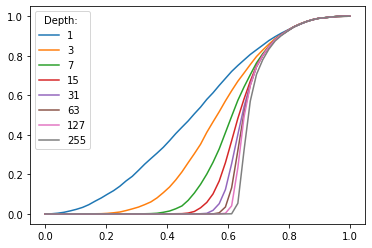
\includegraphics[width=3.5in]{10.png}
\centering
\end{figure}

به نظر می‌رسد احتمال بقا، برای مقادیر
$p$
بزرگتر از حدودا
$0.63$
ناصفر است.

\bibliographystyle{alpha-persian}


\bibliography{main}


\end{document}